%Chapter 5 - Evaluating the MEGA65 project against known risks
%	How exposed to risks is the MEGA65 project july 19?
%	What can be done to reduce the MEGA65 project’s risks?

\chapter{Risk evaluation of the MEGA65 project in July 2018}
\label{Chapter5}
This chapter aims to provide useful advice to the MEGA65 project, with the aim of reducing the project's risk exposure. To achieve this, the detailed snapshot of the project's progress at the point in time of July 2018, shown in Chapter \ref{Chapter4}, is used to evaluate the MEGA65 project's risk levels for risks identified in Chapter \ref{Chapter3}. 

The layout of this chapter is that each risk identified in the risk list is given a section and within each section the MEGA65 project is scrutinised to determine its risk level to that specific risk. Following the risk evaluation, for the identified high risk areas, some advice that could reduce the project's risk level is given. This advice is in the form of alternate solutions or methods of doing things and their potential risk reduction. 

\begin{figure} \begin{center}
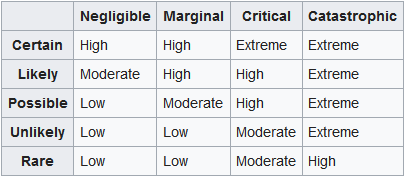
\includegraphics[width=.5\linewidth]{pics/riskmatrix} 
\end{center} 
\caption{Risk matrix showing levels of risk for given likelihood and harm severity.\\}
\label{riskmatrix}
\end{figure}

%----------------------------------------------------------------------------------------
%----------------------------------------------------------------------------------------
\section{Risk evaluation}
\label{evaluation 18}
For each risk identified in the risk list, figure \ref{risk list}, there is a discussion of the factors which may change the risk level and are relevant to the MEGA65 project. These factors could affect the potential damage or the likelihood of the risk.

The risk evaluation of the MEGA65 project is carried out following the guidelines given in \textit{AS ISO 31000:2018 Risk management — Guidelines} 
\cite{RN164} and categorised using the definition of damage listed in the table at the start of Chapter \ref{Chapter3}. The risk is determined using the risk matrix Figure \ref{riskmatrix}.

\subsection{Laws and Regulations}
The MEGA65 products, the MEGAphone and the desktop version, will have to comply with the relevant laws and regulations of the countries in which they are sold in. These laws and regulations are specific to each country, but the general definition and intent of the laws and regulations is similar in lots of places around the world, at least in regard to electronic consumer products. This similarity in laws and regulations comes, in part, from international organisations and standards being adopted or used as a starting point for country specific standards. While the potential damage to a project is catastrophic as it could force a project to be abandoned in the most extreme cases, the uncertainty is fairly low as the laws and regulations are placed in the public domain before being enacted and should be unambiguous. Two cases of laws and regulations causing problems were identified during the case studies. The Raspberry Pi was delayed due to electronic interference testing and the Spectrum Vega was delayed due to age rating testing. While both of these examples are European specific, they similar nature of the laws and regulations of many market places make them relevant for a large portion of the world. \\

The MEGA65 project is rated as a marginal level of damage to the project from a law and regulation related risk. This is due to the projects ability to adapt to change quite well and it doesn't have a strict time or cost constraints. If a product was found to breach electronic interference laws for example, the MEGA65 team would be able to redesign and test the new product with only marginal delays in time and cost. The MEGA65 team is aware of this risk and of the most notable examples of these laws, such as electronic interference and age rating testing, but not of the specific laws of each market they are intending to operate in. The project has indicated that they are intending to carry out specific research into the laws and regulations of certain markets. Until this research has been conducted, the project has been rated at a likely level of probability of occurring.  \\

\begin{tabular}{l|l} % <-- Alignments: l=left, c=centre, r=right
    	\textbf{Category} 	&	\textbf{Rating} \\
      \hline
     Likelihood			&	Likely \\
     Possible Damage 	& 	Marginal \\
     Risk 				&	High		\\	
    \end{tabular}


\subsection{Brexit-like events}
There are no foreseeable Brexit-like events that would be likely to affect the MEGA65 project. Brexit itself is unlikely to affect the MEGA65 project as the project is largely based in Australia, with the desktop version being made in Germany. The potential market for the MEGA65 in the United Kingdom is small and there will likely be some level of agreement with current laws and regulations within the United Kingdom to reduce to the disruption to the market during the transition out of the EU. The project has been rated as unlikely to experience this type of risk. The potential damage to the MEGA65 project was rated as marginal. \\

\begin{tabular}{l|l} % <-- Alignments: l=left, c=centre, r=right
    	\textbf{Category} 	&	\textbf{Rating} \\
      \hline
     Likelihood			&	Unlikely \\
     Possible Damage 	& 	Marginal \\
     Risk 				&	Low		\\	
    \end{tabular}


\subsection{Crowd-funding}
The MEGA65 is considering using crowd-funding to raise funds but importantly they will wait until the design and component selection is complete before launching the campaign.

\subsection{Crowd-funding: contract of sale}
The fact the the MEGA65 team are waiting until much later in the productization process to launch the crowd-funding campaign greatly reduces the risks associated with it. The risk comes from forming a contract of sale between MEGA65 project and backers of the crowd-funding campaign and that contract not being fulfilled. This could lead to legal proceedings against the MEGA65 project. The fact that the MEGA65 project won't launch a crowd-funding campaign until a much later stage in productization means the chance that the MEGA65 project will fail to deliver the product is greatly reduced. This is due to the uncertainty factor being reduced as a lot of the design and component selection is done, as such is not uncertain but certain. The MEGA65 project is rated as having an unlikely probability that it would cause a critical amount of damage to the project. \\

\begin{tabular}{l|l} % <-- Alignments: l=left, c=centre, r=right
    	\textbf{Category} 	&	\textbf{Rating} \\
      \hline
     Likelihood			&	Unlikely \\
     Possible Damage 	& 	Critical \\
     Risk 				&	Moderate		\\	
    \end{tabular}


\subsection{Crowd-funding: currency}
If the MEGA65 team does decide to go the crowd-funding route they will need to decide on what currency to operate in. The risk here is the currency exchange rate drops after receiving the funds and now the actual purchasing power of the funds may be reduced. This risk is increased with time, the longer you hold onto the funds without spending them the more chance the exchange rate will fluctuate. As the MEGA65 team will wait until the product is much further along in the productisation process before crowd-funding this time period will be significantly reduced. There are also some currency which are more stable, in general, and research into these would also reduce the risk by allowing the MEGA65 team to use a stable currency to raise funds in. Another aspect to consider is the currency in which the majority of the funds will be spent i.e. if most of the parts and components are coming from USA companies then it may make sense to use the USD as the crowd-funding currency. The MEGA65 project is rated as unlikely to experience these risks and it would most likely produce a marginal level of damage if it did occur. \\

\begin{tabular}{l|l} % <-- Alignments: l=left, c=centre, r=right
    	\textbf{Category} 	&	\textbf{Rating} \\
      \hline
     Likelihood			&	Unlikely \\
     Possible Damage 	& 	Marginal \\
     Risk 				&	Low		\\	
    \end{tabular}


\subsection{Crowd-funding: failure to meet funding goal}
Due to the funding model of the MEGA65 project their is a lot more flexibility in the way the project moves forward after this event, if it did occur. The MEGA65 project has no strict criteria on cost or time to release and should only suffer a delay in time if it did not reach the predetermined campaign goal of a crowd-funding campaign. The MEGA65 project is rated as having a possible chance of this occurring, this depends heavily on the reception of the MEGA65 products to the public and how much publicity the campaign receives. The MEGA65 project is rated as likely to receive a negligible amount of damage from this event, should it occur. \\

\begin{tabular}{l|l} % <-- Alignments: l=left, c=centre, r=right
    	\textbf{Category} 	&	\textbf{Rating} \\
      \hline
     Likelihood			&	Possible \\
     Possible Damage 	& 	Negligible \\
     Risk 				&	Low		\\	
    \end{tabular}


\subsection{Sourcing old components}
The MEGA65 project plans to use a 3.5" floppy disk drive as a component in the desktop version of the MEGA65. This is because the Commodore 65 prototype featured an internal 3.5" floppy disk drive. This use of old components brings increased risk due to the part not being in mass-production or common usage as such the availability of stock may be limited and the price may increase dramatically if the component is rare or becomes rare. The risk becomes even greater if the component is no longer in production and it needs to be manufactured for the project. This risk also increases with time as it is almost certain, given a long enough time period, that every component will become obsolete and thus expensive to purchase or produce. The MEGA65 is certain to be exposed to this risk. The project is rated as having a marginal amount of damage caused due to the 3.5" inch floppy still being in production and available to purchase. \\

\begin{tabular}{l|l} % <-- Alignments: l=left, c=centre, r=right
    	\textbf{Category} 	&	\textbf{Rating} \\
      \hline
     Likelihood			&	Certain \\
     Possible Damage 	& 	Marginal \\
     Risk 				&	High		\\	
    \end{tabular}


\subsection{Use of 3rd party intellectual property}
The MEGA65 project has exposure to this risk in several areas. Due to the nature of the MEGA65 project, and retro-computing projects in general, being inspired by products from the past, there is commonly intellectual property that the retro project wants to use or imitate to better replicate their inspiration. This is true for the MEGA65 project, being inspired by the Commodore 64 and 65, there are several areas in which being similar to these machine would greatly help the MEGA65 project. They are listed here:

\begin{enumerate}
\item Commodore logo on Commodore key
\item Commodore 64 software including games
\item Commodore 64 character set
\item Commodore 64 BASIC ROM
\item Commodore kernel ROM
\end{enumerate}

\textbf{Commodore logo on Commodore key} \\
The Commodore 64 and 65 featured a special Commodore key with a Commodore icon on it (sometimes referred to as "C="). The MEGA65 desktop form-factor will need a key to function as the Commodore key if it to run Commodore 64 software. It would help users of the MEGA65 understand what the key is used for if the icon on it made users think of the Commodore key. An exact copy of the Commodore icon would fulfil this perfectly but it is a trademark, along with the Commodore name, as such they both carry risk in using. The MEGA65 project is certain to encounter this risk and there is a critical amount of potential damage that could be caused in using the Commodore icon. \\

\begin{tabular}{l|l} % <-- Alignments: l=left, c=centre, r=right
    	\textbf{Category} 	&	\textbf{Rating} \\
      \hline
     Likelihood			&	Certain \\
     Possible Damage 	& 	Critical \\
     Risk 				&	Extreme		\\	
    \end{tabular} \\ \\


\textbf{Commodore 64 software including games}\\
The software in question is specifically applications such as games, text editors or other a productivity software as some non-exhaustive examples, not the kernel or BASIC environment software. The MEGA65 aims to be compatible with as many Commodore 64 software titles as possible. This allows a more authentic experience for those seeking to recreate their Commodore 64 experiences. To achieve this the MEGA65 needs software to run on it and specifically it needs the software from the home computer era, created for the Commodore 64, to truly recreate the experience. This software is intellectual property as such its use without an agreement brings risks from legal action taken by the IP holders to protect their property. The MEGA65 project is planning on only including with their products, 3rd party software with which they have implicit agreement from the rights holders to use their intellectual property. This could either be from the rights holders stating their software is free to use to the public or through the MEGA65 team reaching out to the rights holders and them forming an agreement. Because of this, the MEGAG65 project has been rated as having a rare likelihood of experiencing this event. 

The potential damage caused by this event comes in three parts: \\
a) The loss of user experiences and value to the users of the MEGA65 \\
b) The loss of time spent removing games from memory, documentation and promotional material \\
c) The loss of time and money responding to legal challenges and rulings \\


The MEGA65 project would be expected to experience negligible damage from a) and b). The damage from c) would be marginal as the MEGA65's market is likely to be small so any potential losses to rights holders would also be small which would suggest and legal ruling awarding the rights holders for loss of earnings would also be small. \\

\begin{tabular}{l|l} % <-- Alignments: l=left, c=centre, r=right
    	\textbf{Category} 	&	\textbf{Rating} \\
      \hline
     Likelihood			&	Rare \\
     Possible Damage 	& 	Marginal \\
     Risk 				&	Low		\\	
    \end{tabular} \\ \\


\textbf{Commodore 64 character set}\\
The MEGA65 requires a set of character bitmaps stored in memory, this is used to display text on the screen. The Commodore 64 character set would be ideal for this purpose as it is readily available from numerous website and would help the MEGA65 replicate the Commodore 64 more closely. The Commodore 64 character set is intellectual property, as such its use in the MEGA65 project brings risk. The MEGA65 project currently does not have an agreement to use the Commodore 64 character set. There is a certain likelihood of this occurring and a marginal level of damage that could occur. \\

\begin{tabular}{l|l} % <-- Alignments: l=left, c=centre, r=right
    	\textbf{Category} 	&	\textbf{Rating} \\
      \hline
     Likelihood			&	Certain \\
     Possible Damage 	& 	Marginal \\
     Risk 				&	High		\\	
    \end{tabular} \\ \\


\textbf{Commodore 64 BASIC ROM}\\
The MEGA65 requires a BASIC ROM which will provide the BASIC environment into which it boots into on start up. This ROM, of which there are numerous versions specific to differing versions of BASIC, should be a ROM which provides the greatest amount of compatibility with Commodore 64 and 65 software, as the user will derive greater facility from it. The Commodore 64 BASIC ROM would be the ideal candidate but it is intellectual property and will attract risk if used. The MEGA65 project currently does not have an agreement to use the Commodore 64 BASIC ROM. The MEGA65 project is certain to experience this risk with the potential damage being critical. \\

\begin{tabular}{l|l} % <-- Alignments: l=left, c=centre, r=right
    	\textbf{Category} 	&	\textbf{Rating} \\
      \hline
     Likelihood			&	Certain \\
     Possible Damage 	& 	Critical \\
     Risk 				&	Extreme		\\	
    \end{tabular} \\ \\


\textbf{Commodore 64 kernel ROM}\\
The MEGA65 requires this ROM for basic functionality and it is of critical importance to the compatibility of the MEGA65 with Commodore 64 software that the kernel used function as the Commodore 64 kernel does. The ideal candidate kernel if only the functionality of the MEGA65 is considered, is the Commodore 64 kernel. This kernel is intellectual property as such it will attract a risk if used without an agreement with the rights holder. The MEGA65 project does not currently have an agreement with the rights holder. The potential damage from this risk is from the rights holder undertaking legal action against the MEGA65 project. The likelihood of this event occurring is considered unlikely as the ROM has been available online for decades with no noticeable attempt to control its distribution. The potential damage is catastrophic as the MEGA65 could not function without a kernel and if the Commodore 64 kernel was not able to be used suddenly, the MEGA65 would effectively be useless until a replacement was found. \\

\begin{tabular}{l|l} % <-- Alignments: l=left, c=centre, r=right
    	\textbf{Category} 	&	\textbf{Rating} \\
      \hline
     Likelihood			&	Unlikely \\
     Possible Damage 	& 	Catastrophic \\
     Risk 				&	Extreme		\\	
    \end{tabular}


\subsection{Open-source business}
The MEGA65 project will be exposed to this risk, which is related to competitors being able to produce and sell the MEGA65 with no money being generated for the MEGA65 team. This means it can be harder to operate as a traditional electronics business in which its products are propriety and they can discourage competitors using there designs with legal challenges. The MEGA65 project is likely to not have a large market, as such the cost to enter the market is quite high compared to the potential profits. This will help reduce the likelihood of this occurring as long as the assumption that the MEGA65's market is small, remains true. The MEGA65 project is rated as possible for the likelihood of this occurring and a critical level of damage could be caused. \\

\begin{tabular}{l|l} % <-- Alignments: l=left, c=centre, r=right
    	\textbf{Category} 	&	\textbf{Rating} \\
      \hline
     Likelihood			&	Possible \\
     Possible Damage 	& 	Critical \\
     Risk 				&	High		\\	
    \end{tabular}


\subsection{Loss of intellectual property}
This relates to the loss of agreement to use intellectual property that is require for the MEGA65. This occurred the most dramatically in the Vega Plus case study where the CTO left RCL, the makers of the Vega Plus, and refused to let them use his prototype. The MEGA65 is entirely shielded from this due to the open-source nature of the designs used throughout the entire project. No team member owns any part of the design as such they cannot withdraw their agreement for MEGA65 to use it. The MEGA65 project is rated as having a rare chance (the lowest) of occurring this event and of it doing negligible damage.  \\

\begin{tabular}{l|l} % <-- Alignments: l=left, c=centre, r=right
    	\textbf{Category} 	&	\textbf{Rating} \\
      \hline
     Likelihood			&	Rare \\
     Possible Damage 	& 	Negligible \\
     Risk 				&	Low		\\	
    \end{tabular}


\subsection{Supplier failure}
The MEGA65 is exposed to this risk whenever they purchase from a 3rd party. The desktop version which is undergoing physical development with MEGA, and is intended to enter a pre-production stage of development soon, is rated as having a marginal rating of potential damage should this event occur. This is due to the fact the while the desktop version is in pre-production it will have several different components being manufactured by different suppliers. These components need to be assembled together to form the MEGA65 desktop version once they are all complete. A delay in any of the components could cause a time delay in the overall construction of the MEGA65 desktop version preproduction run. A delay could also incur additional costs if a new manufacturer has to be found or if there are storage costs caused by the delay. The desktop version is rated as having a unlikely chance of this event occurring as the suppliers chosen are established businesses. The other MEGA65 form factor, the MEGAphone, is undergoing the alpha stage of production as such the purchases are currently small as they are focused on a single prototype. This reduces the potential damage to negligible during this phase. As the MEGA65 products enter full production the risk increases. The MEGA65 team members are aware of this risk and of the preference to use established businesses and undertake due diligence. With all the above factors considered, the MEGA65 project is rated as having a marginal level of potential damage and a unlikely chance of this event occurring. \\

\begin{tabular}{l|l} % <-- Alignments: l=left, c=centre, r=right
    	\textbf{Category} 	&	\textbf{Rating} \\
      \hline
     Likelihood			&	Unlikely \\
     Possible Damage 	& 	Marginal \\
     Risk 				&	Low		\\	
    \end{tabular}


\subsection{Open-source fair use}
This should not be an issue for the MEGA65 project as all of the open-source components are created by project members or freely available to be used in projects such as the MEGA65. \\

\begin{tabular}{l|l} % <-- Alignments: l=left, c=centre, r=right
    	\textbf{Category} 	&	\textbf{Rating} \\
      \hline
     Likelihood			&	Rare \\
     Possible Damage 	& 	Negligible \\
     Risk 				&	Low		\\	
    \end{tabular}


\subsection{Physical production problems}
The MEGA65 project is exposed to this risk in both its form-factors. The desktop version will require physical mechanical components such as a keyboard and case. Both of these components have the potential to experience problems during manufacturing, assembly or testing. These problems such as incorrect material, incorrect size, rough edges or wrong shape to name a few, could potentially cost the project lost time and money. The desktop version has a possible chance of this event occurring and a negligible level of potential damage. The MEGAphone form factor which is much less advanced in its physical design compared to the desktop version, is more exposed to this risk. This is due to the case design having not been created or tested as well as the use of touch screen and button interface, all of which add complexity to the design. The potential damage for the overall project is rated as marginal and it has a possible chance of occurring. \\ 

\begin{tabular}{l|l} % <-- Alignments: l=left, c=centre, r=right
    	\textbf{Category} 	&	\textbf{Rating} \\
      \hline
     Likelihood			&	Possible \\
     Possible Damage 	& 	Marginal \\
     Risk 				&	Moderate \\	
    \end{tabular}


%----------------------------------------------------------------------------------------
%----------------------------------------------------------------------------------------
\section{Recommendations for reducing the MEGA65 project's risk exposure}
\label{recommendations}
In this section, practical, actionable advice will be given on how the MEGA65 project can reduce their exposure to the risks identified in Chapter \ref{Chapter3}. Using the risk evaluation of the MEGA65 project as of July 2018, as a starting point, this section aims to reduce the risk by focusing on the highest risk areas and suggesting strategies to reduce that risks.

\subsection{Laws and Regulations}
The MEGA65 project is aware of the need to undertake research into the laws and regulations of the specific markets into which they want to sell the MEGA65. To reduce their risk they must undertake aforementioned research. The potential damage to the MEGA65 project is increased the further the development goes forward without this research. Assuming the research is conducted the likelihood is reduced to rare and a potential risk marginal if the research is conducted in a timely manner.

\subsection{Sourcing old components}
The MEGA65 projects use of floppy disk drives opens up the potential for damage in the future if the become obsolete (which they arguable are already). As they are manufactured less and become rarer, their unit price would be expected to increase. To compensate for this a large inventory of the disk drives could be sourced much earlier than required for production. This could bring twofold benefits in the unit price may come down with a large unit number purchase and the MEGA65 is shielded from component volatility in the medium term (until the stocked drives run out). The downside to this strategy is storage costs as well as increase upfront costs in purchasing the drives.

\subsection{Use of 3rd party intellectual property}
The use of 3rd party software has opened up the MEGA65 project to some high risks. The use of the software is almost unavoidable in cases, if the MEGA65 is to be a true innovation of the Commodore 65 and Commodore 64 compatible. The main areas identified above are the Commodore icon on the Commodore keyboard key and the ROMs required for Commodore 64 compatibility: the character set ROM, BASIC ROM and the kernel ROM. The only options to reduce the risk are to either entered into an agreement with the rights holder and barring that simple not use them in the MEGA65. Suitable replacements may be found in some cases. The Commodore icon could potential be changed to a MEGA65 inspired design. The character set, while being closely linked to the Commodore 64 experience, could be swapped for another more readily available set. The kernel and BASIC ROM are less likely to have suitable replacements readily available. Another strategy would be to create the ROMs within the MEGA65 project. This would completely eliminate the potential risk, as long as the replacements didn't break any copyright laws. 

\subsection{Open-source business}
This risk increases with MEGA65's popularity and market size. At a certain threshold of unit sales other businesses will consider manufacturing the MEGA65 from the open-source designs and selling it themselves. This will not generate any revenue for the MEGA65 team and may be a problem in the long term, depending on the MEGA65's popularity. It may be worth trademarking the MEGA65 name and then later licensing its use to generate profit. The MEGA65 team should also consider branching out into accessories for the MEGA65 as a strategy for dealing with this risk. Dr. Paul Gardner-Stephens and other core team members could also consider commissioned advisory roles and presentations as another strategy. 

